\documentclass{article}
\usepackage[utf8]{inputenc}

\title{Εύρεση Συνολικόυ Συντελεστή Ασφαλείας 
\\(με χρήση συντελεστή μορφής)}
\author{Για τον κώδικα Latex, ενημερώσεις και προτάσεις:
}
\date{}
\usepackage{graphicx}

\usepackage[utf8]{inputenc}
%allow simultaneous greek and english input
\usepackage[greek,english]{babel}
\usepackage{alphabeta}

\begin{document}

\maketitle
\tableofcontents
\section{Introduction}


%%1) na valo dipla se kathe megethos ena velaki analoga me to an i ayksisi toy megethoys ayksanei i meiwnei tin sinoliki antohi toy ajona se taseis 
%%2) na hromatiso katalila to kathe megethos analoga me to an einai anagkaio gia to orio plastikis i dinamikis thraysis i kai gia ta dio 
%%3) Na balo dipla apo ton kathe tipo tis monades toy tipoy ?
%4) Na valo ta pinakakia me ta esb ktlp sto telos kathws kai ta shediagramata ta opoia ehoyne olin tin diadikasia periliptika 
%5) Na valw sto telos aytoy toy pdf toys pinakes 2.1a-z
%6) Πως καταλαβαίνουμε στο κ1deff ποιοί χάλυβες είναι σε υψηλή περιεκτικότητα σε CRNIMO kai poioi oxi?
%7) Σε όλες τις ασκήσεις θεωρούμε το dB ;iso me 16mm ?
%8) Ποτε να βρίσκουμε το Κ1deff μέσω του διαγράμματος και πότε μέσω των τύπων?
%9) Μέτα την ευρεση του Κ1def βρίσκουμε 
%10) Γιατί στο παράδειγμα 1 στον υπολογισμό του συντελεστή α
%11) Να προσθέσω στην αρχή? το κομμάτι που βρίσκω τις ονομάστικές τάσεις
%12) Όταν προσθέσω το κομμάτι στο οποίο δίνονται οι ονομαστικές τάσεις να γράψω οτι οταν οι ροπές δίνονται σε Nm πρέπει να τις μετατρέψω σε Nmm
%13) Na prosthesw tin metafrasi ton halivon apo to germaniko DIN sto europaiko ph St37 = S235JR (Mporw na to valw pano stis idi iparhouses eikones)


Nom;izv meta thn selίδα 11 θα έπρεπε να υπάρχει το σ_bFK


Intro:Σε διάφρορα σημεία στην μεοδολογία χρειάζεται να ξέρουμε το esb ess eszdw κτλπ. Αυτά τα βλέπουμε απο τα πινακάκια στην αρχή των σημειώσεων του μιχαηλίδη.(Παραθάτωνται στο τέλος του PDF(δεν έχουνε μπεί ακόμα))
\begin{itemize}
    \item Πολλές μεταβλητές έχουνε τον δείκτη σ και τ (πχ $α_σ,τ$). Ουσιαστικά αυτή η μεταβλητή εκφράζει το ίδιο μέγεθος στην περιπτωση της κάμψης και της στρέψης αντίστοιχα
    \item 1kp = 9.8066 N
\end{itemize}
\\
\\

\section{\textbf{\huge $σ_Β$, $σ_S$, $σ_{zdW}$, $σ_{bW}$, $τ_{tW}$ },   (Όριο θραύσεως για την διάμετρο $d_B$, Όριο πλαστικής παραμόρφωσης, Επιτρεπώμενο ημιέυρος εναλλασόμενου εφελκυσμού, κάμψης και στρέψης.)}
Για όλες τις ασκήσεις θεωρούμε το $d_B$ ίσο με 16mm (mallon, na to rotisw)
\includegraphics[width=\linewidth]{0.1.png}


\includegraphics[width=\linewidth]{0.2.png}

\section{\textbf{\huge $a_σ$, $α_τ$  }    (Συντελεστής μορφής της εγκοπής) } 
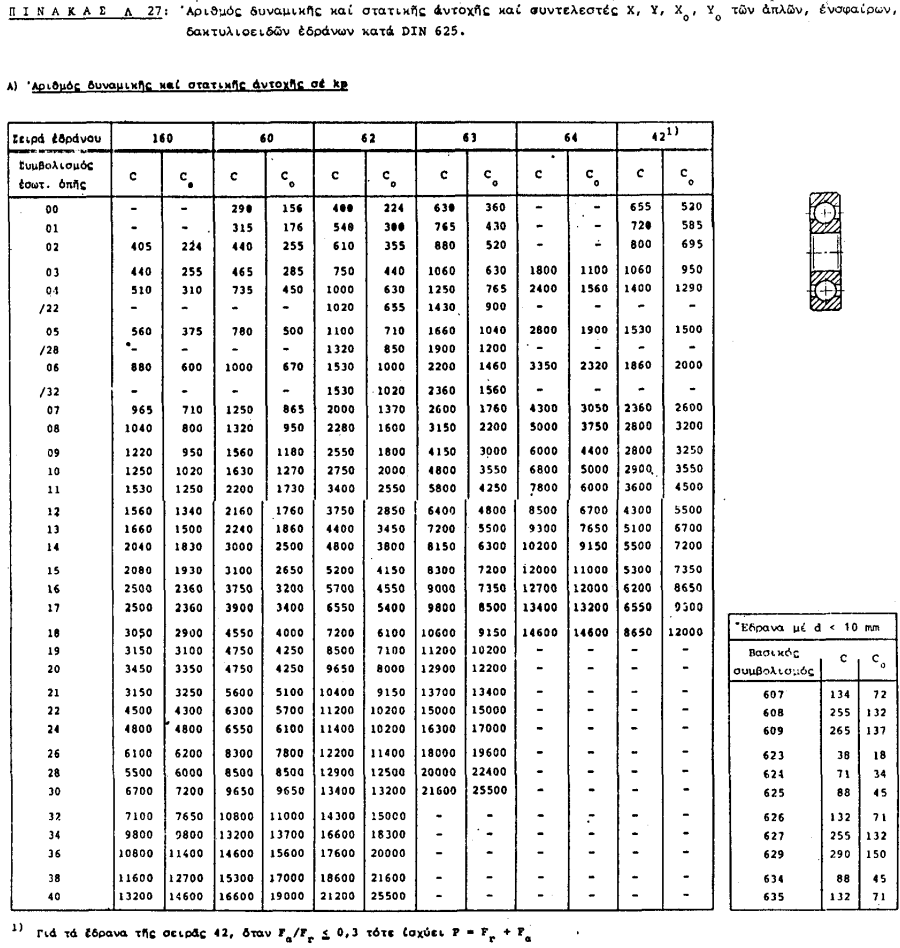
\includegraphics[width=\linewidth]{1.png}
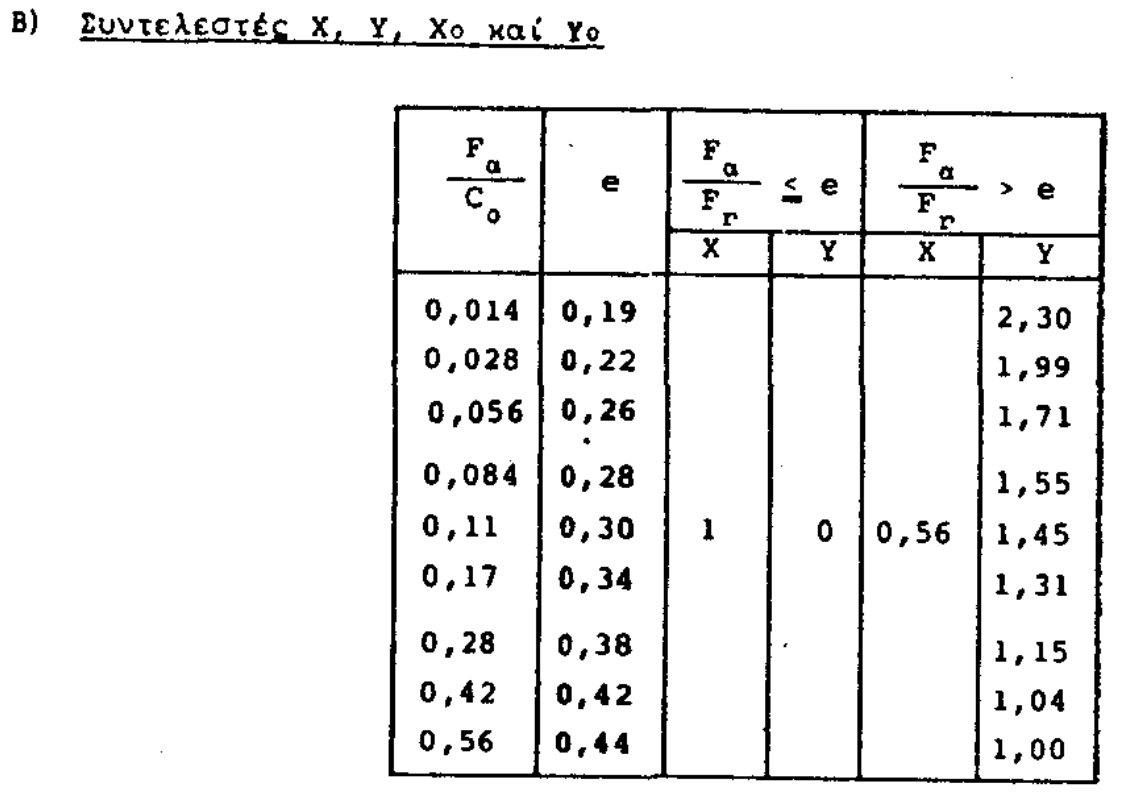
\includegraphics[width=\linewidth]{2.png}
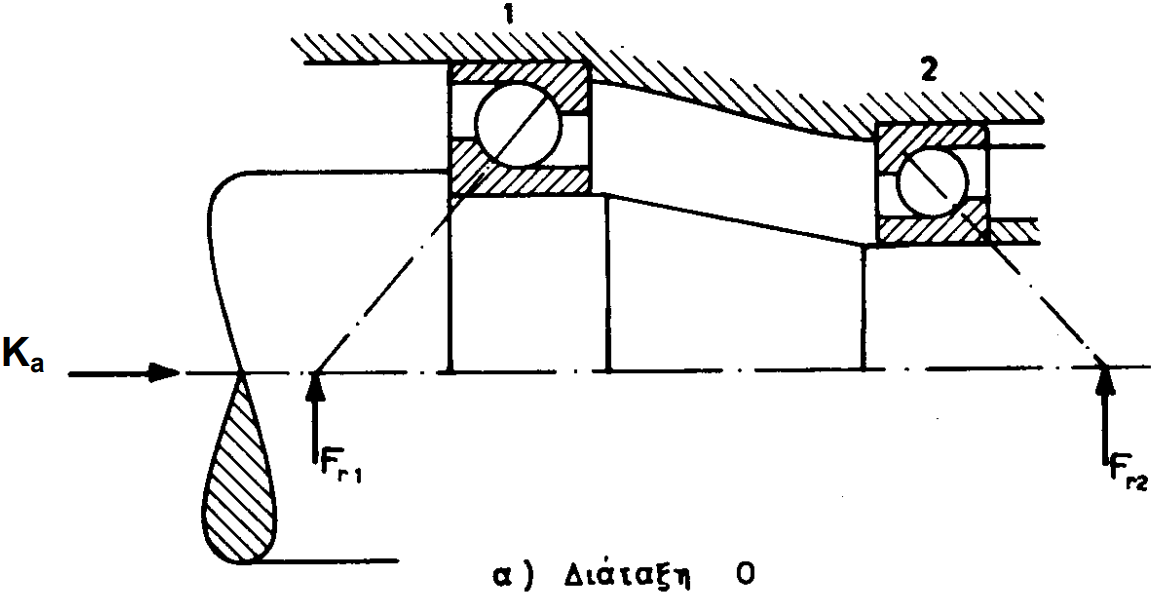
\includegraphics[width=\linewidth]{3.png}
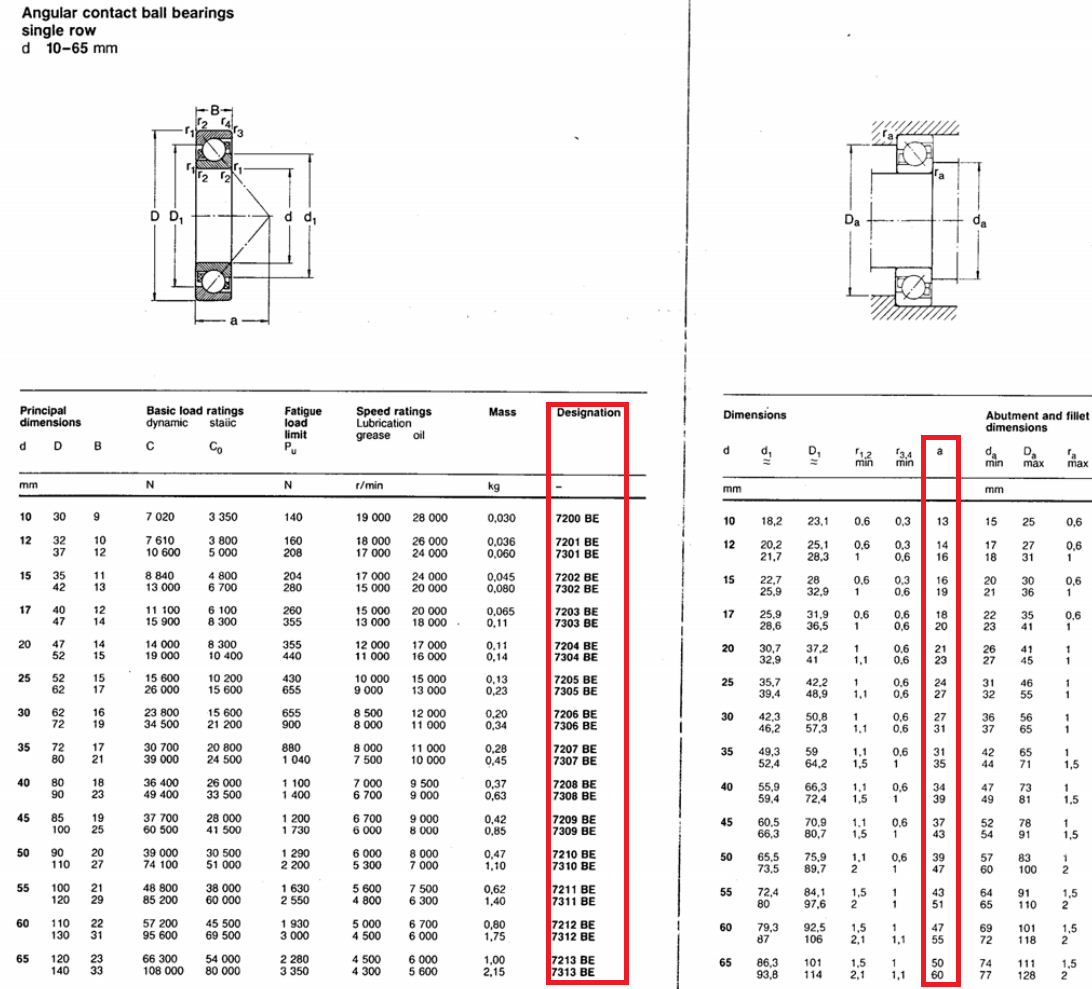
\includegraphics[width=\linewidth]{4.png}
\section{\textbf{\huge G΄}  (Σχετική Πτώση Τάσης) }
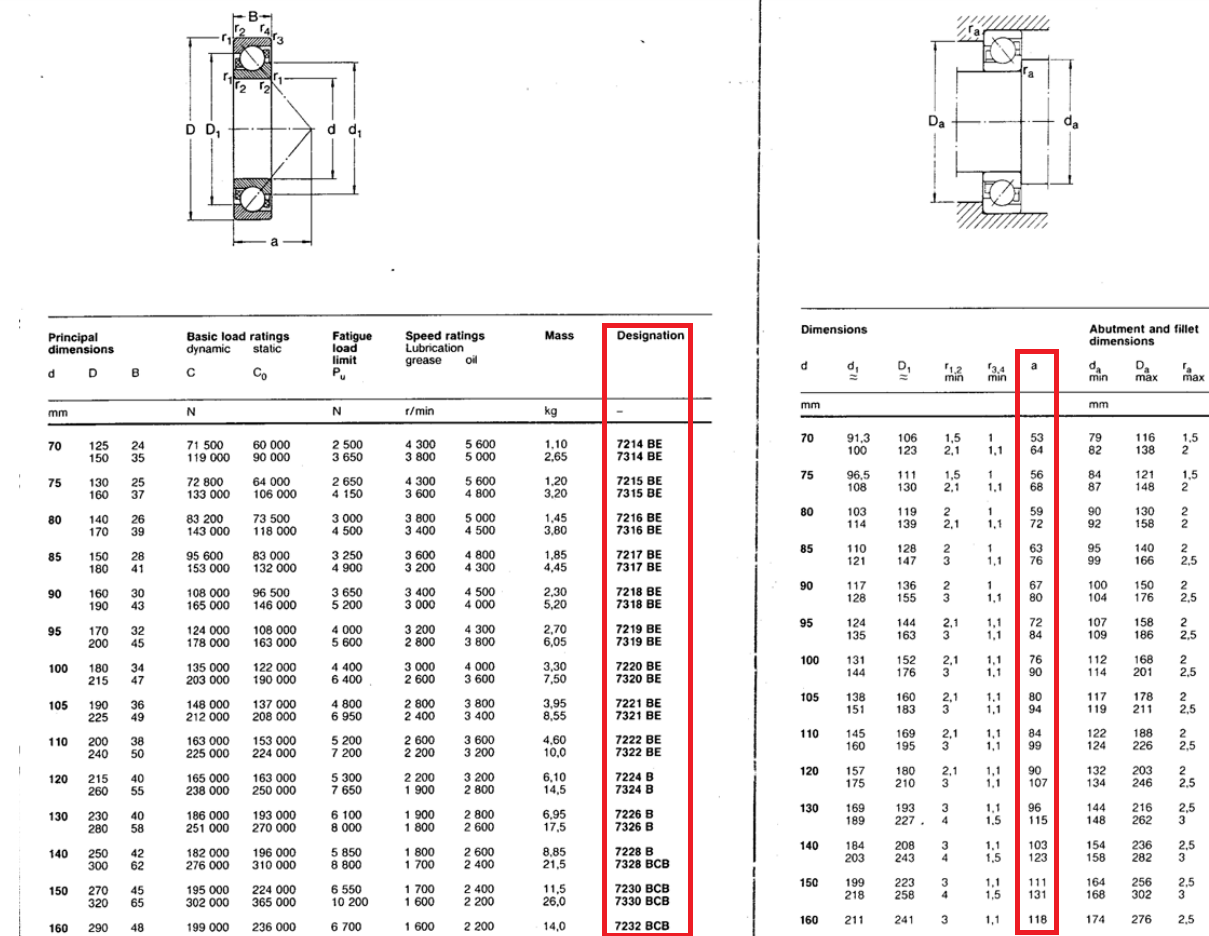
\includegraphics[width=\linewidth]{5.png}


\\
\\



\section{\textbf{\huge $K_1(deff)$ }   (Συντελεστής επίδρασης μεγέθους στην θερμική κατεργασία) }
Παρακάτω ζητήται η μεταβλητή D-eff. Το d-eff είναι η διάμετρος με την οποία κατασκευάστηκε ο αξονας μας(η διάμετρος η οποία βγήκε απο το εργοστάσιο όχι αυτήν στην οποία μπορεί να κόψαμε τον άξονα μας. Αυτό γιατί μπορεί ο άξονας μας να είχε δεχτεί επιφανειακές κατεργασίες οι οποίες επηρεάζουνε την συμπεριφορά του. D-eff είναι η διάμετρος στην οποία έγινε η θερμική κατεργασία.
\\


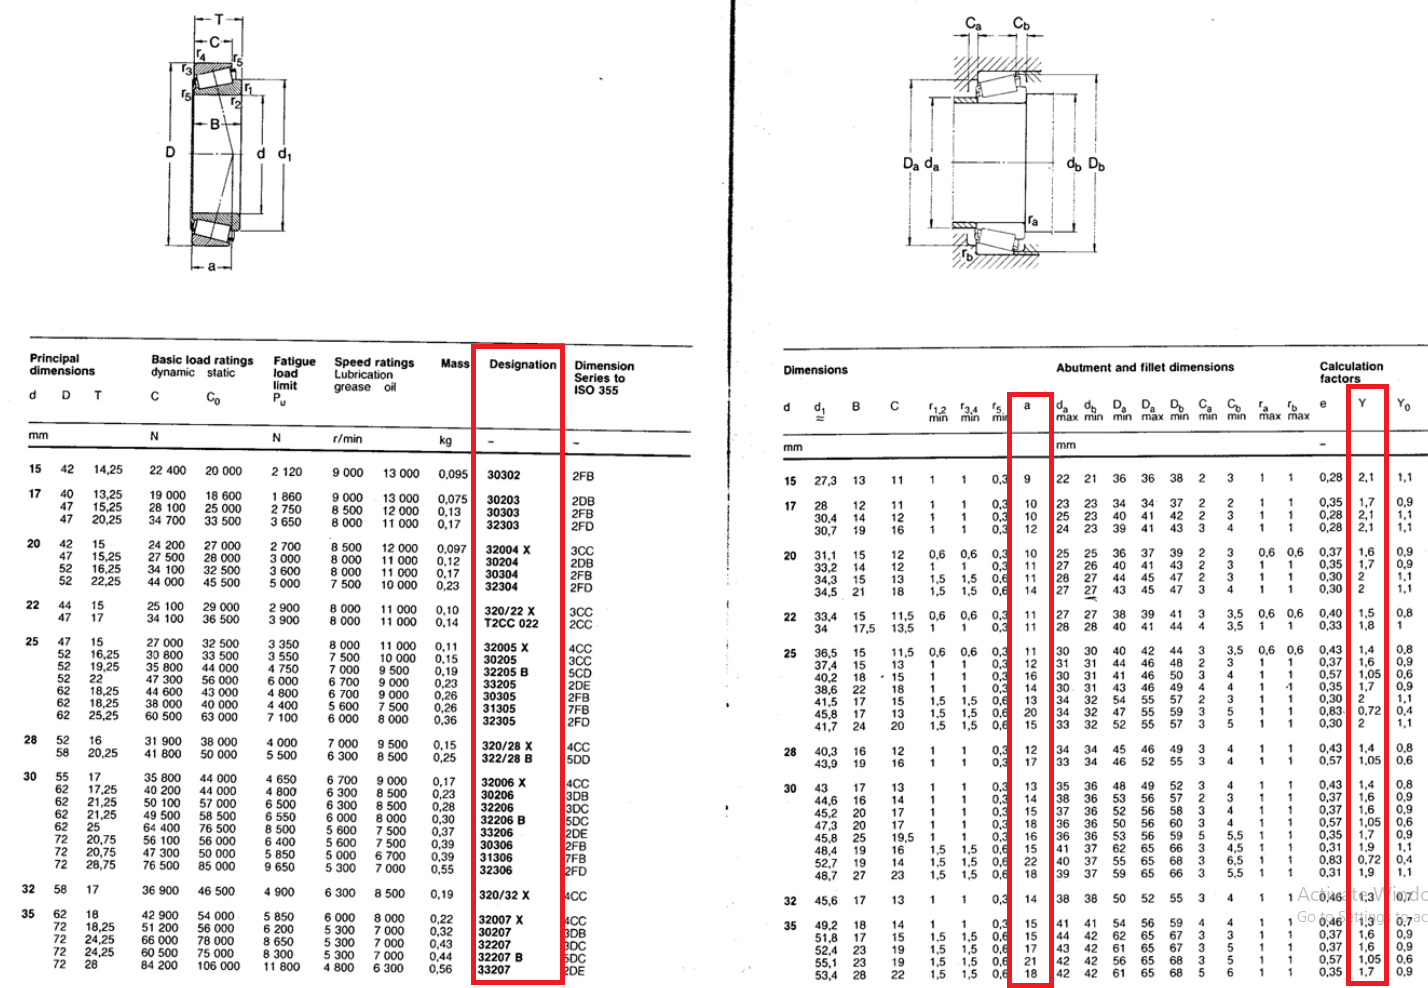
\includegraphics[width=\linewidth]{6.png}
\\
\\
\\

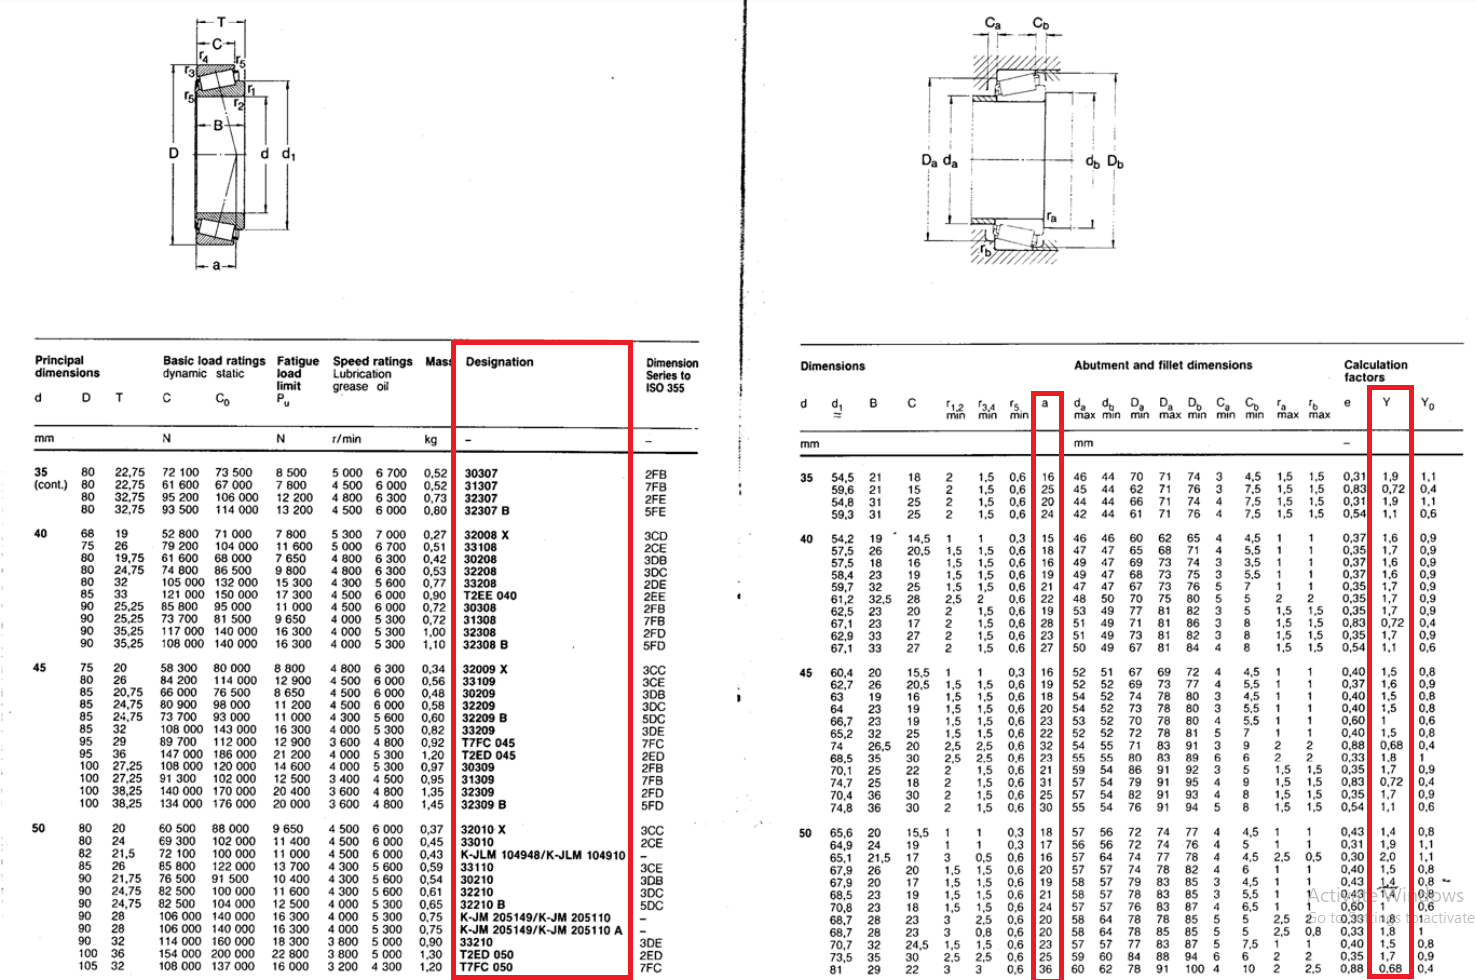
\includegraphics[width=\linewidth]{7.png}
\section{\textbf{\huge $n$}  (Συντελεστής δυναμικής αντιστήριξης)} 
Το $σ_s(d_B)$ το οποίο χρησιμοποιόυμε για να βρούμε το $σ_s(d)$ είναι αυτό το οποίο βρήκαμε απο τα πινακάκια στην αρχή της διαδικασίας. Ουσιαστικά δηλαδή είχαμε το όριο ενός δοκιμίου διαμέτρου 16mm σε πλαστική παραμόρφωσή και με αυτήν την πράξη βρίσκουμε το όριο του δικού μας άξονα σε πλαστική παραμόρφωση.
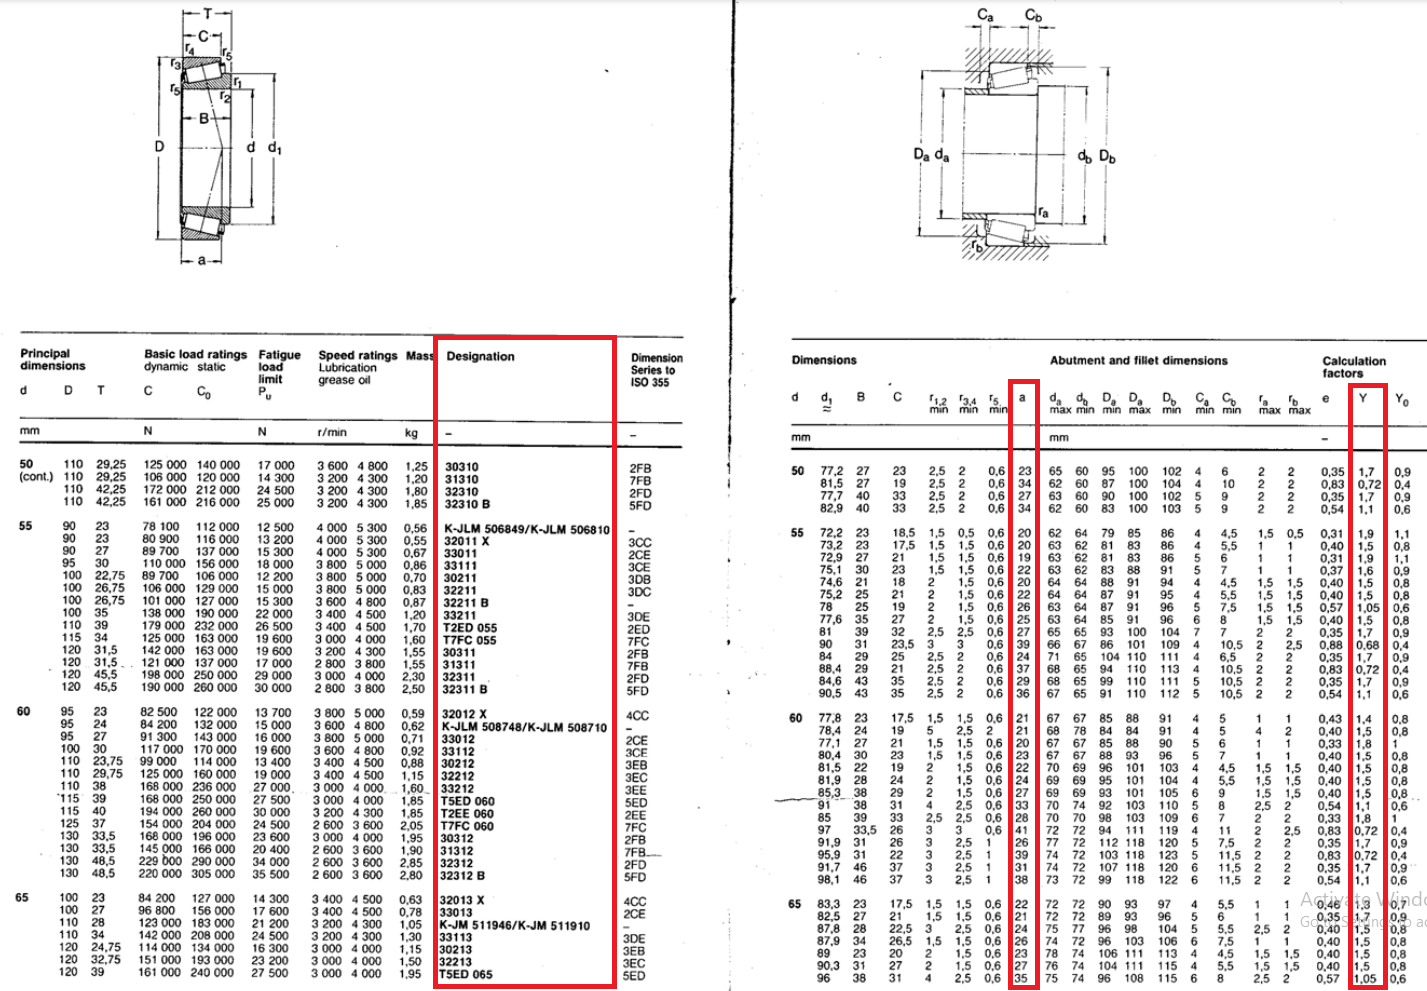
\includegraphics[width=\linewidth]{8.png}

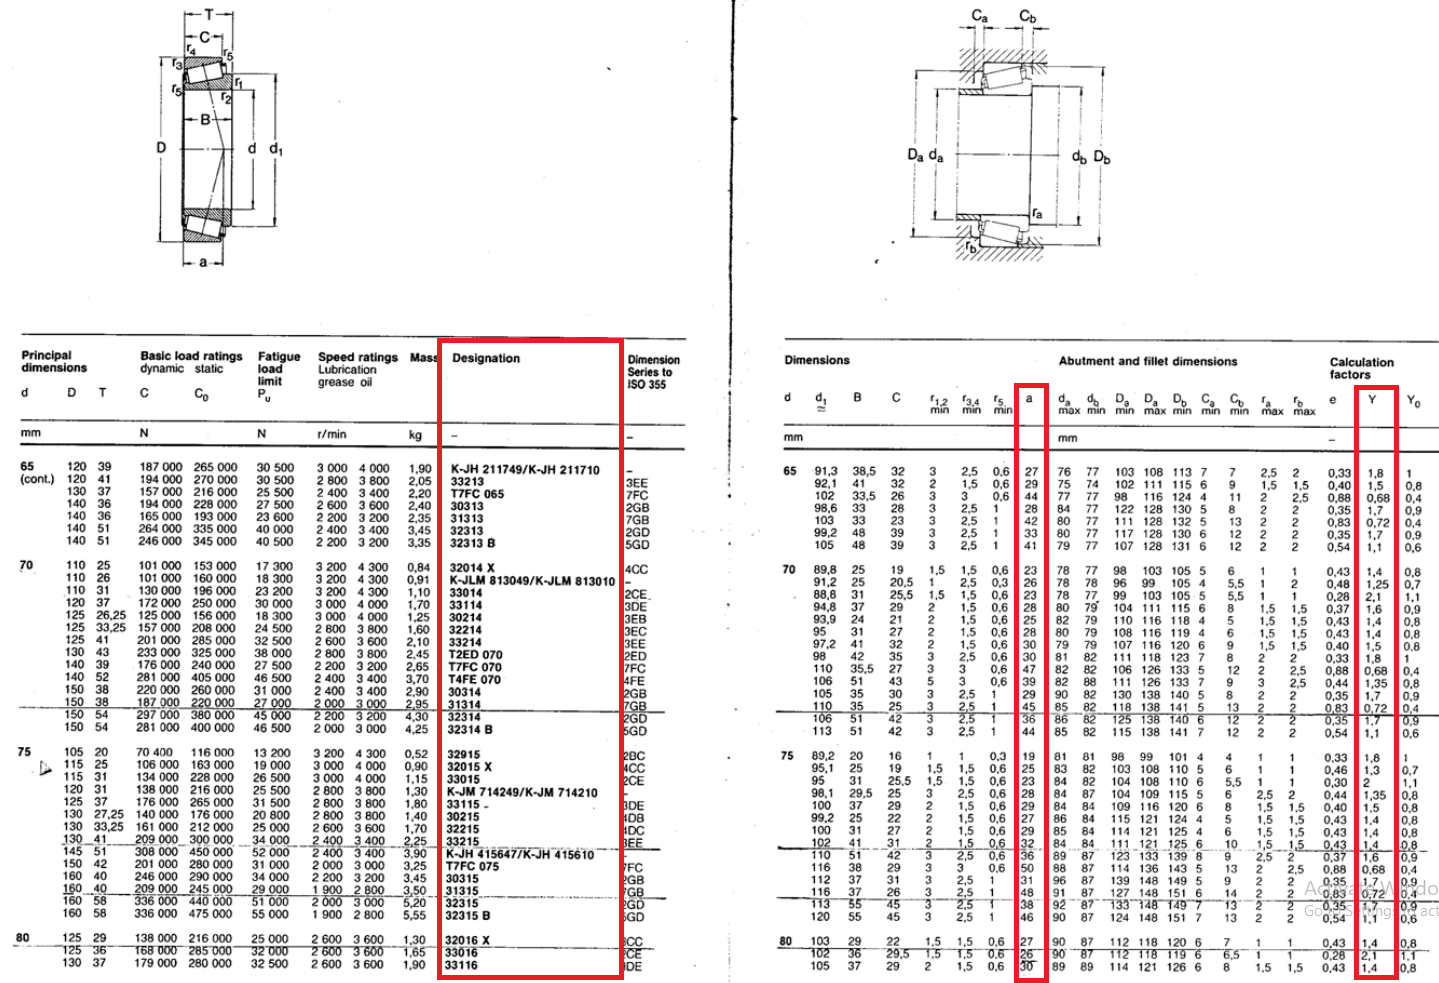
\includegraphics[width=\linewidth]{9.png}
\section{\textbf{\huge $β_σ_τ$}   (Συντελεστής Εγκοπής)}
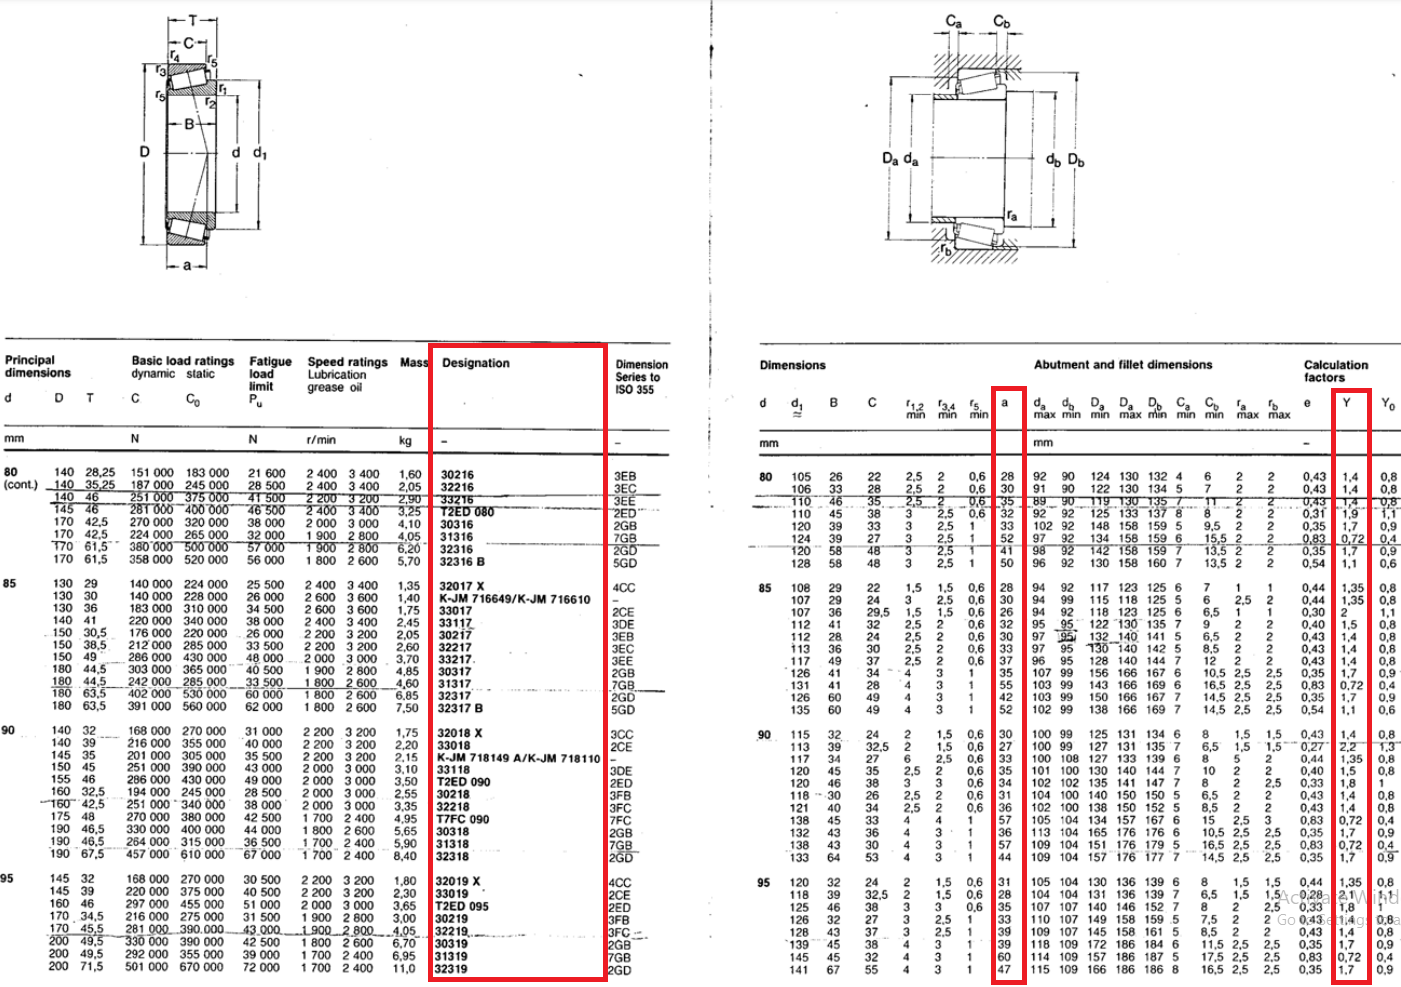
\includegraphics[width=\linewidth]{10.png}
\section{\textbf{\huge $K_2(d)$}  (Συντελεστής Επίδρασης Μεγέθους) }
Το d το οποίο εμφανίζεται εδω πέρα είναι το μικρό d του άξονα 
\\
\includegraphics[width=\linewidth]{11.png}
\includegraphics[width=\linewidth]{12.png}  
\section{\textbf{\huge $K_F$ }  (Συντελεστής Τραχύτητας) }
 Αν μας δίνεται το Rt και όχι το Rz τότε θέτουμε αυθαίρετα οτι Rz = Ρτ η οποία είναι και η χειρότερη περίπτωση 
 \\
\includegraphics[width=\linewidth]{13.png}
\section{\textbf{\huge $K_V$ }  (Συντελεστής Αύξησης Επιφανειακής Αντοχής) }
\includegraphics[width=\linewidth]{14.png}
\section{\textbf{\huge $K__σ_,_τ$}   (Συνολικός Συντελεστής Επίδρασης Εγκοπής) }
\includegraphics[width=\linewidth]{15.png}
\section{\textbf{\huge $K_2_F$ }    (Συντελεστής Στατικής Αντιστήριξης) }
\includegraphics[width=\linewidth]{16.png}

\includegraphics[width=\linewidth]{17.png}
\section{\textbf{\huge $γ_F$}    (Συντελεστής Αύξησης του ορίου πλαστικής παραμόρφωσης) }
\includegraphics[width=\linewidth]{18.png}
\section{\textbf{\huge $σ_z_d_F_K$, $σ_b_F_K$, $σ_t_F_K$}    (Επιτρεπώμενες τάσεις σε εφελκυσμό, θλίψη) }
\includegraphics[width=\linewidth]{19.png}
\section{\textbf{\huge $σ_m_v$,  $τ_m_v$ }       (Ισοδύναμη ορθή μέση τάση και ισοδύναμη εφαπτομενική μέση τάση)  }
\includegraphics[width=\linewidth]{20.png}
\includegraphics[width=\linewidth]{21.png}

\ Τα eszdW, esbW kai taftw βρίσκονται απο τους πίνακες 2.1a-z στην αρχή του pdf του μιχαιλίδη(Υπάρχουν και στο τέλος αυτόυ του pdf(δεν έχουνε μπεί ακόμα))
\\
\section{\textbf{\huge $σ_z_d_K$, $σ_b_W_K$, $τ_t_W_K$}      (Επιτρεπώμενο ημιέυρος για εναλλασσόμενη καταπόνηση) }
\includegraphics[width=\linewidth]{22.png}
\section{\textbf{\huge $ψ_z_d_σ_K$, $ψ_b_σ_K$, $ψ_τ_K$ }   (Συντελεστής καταπονήσεως σε εφελκυσμό/θλίψη, κάμψη και στρέψη ανάλογα) }
\includegraphics[width=\linewidth]{23.png}
\section{\textbf{\huge $σ_z_d_A_D_K$ , $σ_b_A_D_K$ , $σ_τ_A_D_K$}     (Επιτρεπώμενο ημιεύρος τάσεων για δυναμική καταπώνηση γενικής μορφής με εφελκυσμό/θλίψη, κάμψη, στρέψη)}
Σε αυτό το σημειίο πρέπει να βρούμε ποιά απο τις δύο περιπτώσεις φόρτισης θα πάρουμε (F1 ή F2) και σε ποιά απο τις τρείς περιοχές φόρτισης βρίσκεται ή άτρακτος.
\\
\\

\includegraphics[width=\linewidth]{24.png}

\includegraphics[width=\linewidth]{25.png}
\section{\textbf{\huge } Διάγραμμα Smith }
\includegraphics[width=\linewidth]{26.png}
\section{\textbf{\huge $S_D$ }    (Συντελεστής Ασφαλείας για δυναμική θράυση) }
\includegraphics[width=\linewidth]{27.png}
\section{\textbf{\huge  $S_F$}     (Συντελεστής Ασφαλείας για πλαστική παραμόρφωση) }
\includegraphics[width=\linewidth]{28.png}

\includegraphics[width=\linewidth]{29.png}



\end{document}
